\chapter{The MAC layer}

\section{Introduction}

The MAC layer handles access to the same medium, avoiding collisions that cause
waste of time.
It has the following goals:
\begin{itemize}
\item Efficency in bandwith use
\item Avoid collisions (resilience)
\item Fairness
\item Robustness: the protocol should be decentralized
\item Protocols easy to implement
\end{itemize}

\paragraph*{Typologies} The MAC layer has different typologies. As a matter of
fact, it offers different
ways to share the channel: \textbf{TDMA} (\textit{time division}), \textbf{FDMA}
(\textit{frequency division}), \textbf{CDMA} (\textit{time division}).
\paragraph*{Random access} MAC provides two way to randomly access the channel,
with \textbf{CSMA}
(\textit{carrier sense multiple access} and MACA (\textit{multiple access with
  collision avoidance}).
\paragraph*{Other protocols} There are also ``taking turns'' MAC protocols, that
basically carries out a
polling scheme.

\subsection{Wired vs Shared Channel}

When the channel is a cable it's easier, because you just have to listen to it
before trasmitting any data (this techinque is called CSMA, \textit{Carrier
  sense  multiple access}\footnote{As an additional note, with CSMA you can even listen  when a collision happens.}): for example with ethernet you can check what you've sent and check if a collision happened. In a wireless environment this is not possible, because when you're transmitting you can't receive, otherwise you'll end up having a collision, but you can check if a package has arrived to the destination with the ACKs\footnote{
  In wireless communications TCP packets are split into smaller packages of 100bytes each one when thay arrive to the MAC layer: the ACKs are generated during transmission for the MAC layer and when a complete TCP packet is sent the receiver will generate a TCP response. Any TCP packet can generate one o more MAC packet, allowing the MAC layer to hide some losses to the top protocol. N.B.: this is not true for ad-hoc communications though.
}.

\section{MAC Layer approaches}

There are different ways the MAC layer can approach the access to the medium,
and these are:
\begin{itemize}
\item Random
  \begin{itemize}
  \item without carrier sensing (such as Aloha, Slotted Aloha)
  \item with carrier sensing (CSMA, CSMA/CD, MACAW)
  \end{itemize}
\item Controlled
  \begin{itemize}
  \item centralized (FDMA, TDMA, CDMA)
  \item distributed
  \end{itemize}
\end{itemize}

\subsection{Aloha}

This protocols was used to communicate between Hawaii islands. It doesn't have
synchronization, and the total thoughput of this protocols is $\frac{1}{2}e$

\subsubsection{Slotted Aloha}

This version of Aloha has time divided slots: every transmission has to stay in
a defined time slot, that is not easy to do but it's possible. In case of a
collision, a retransmission occurs with a probability $P$.

\paragraph*{Thoughput} The thoughput of this Aloha version with synchronization
is $\frac{1}{e}$

\subsubsection{Considerations about Aloha protocols}

In general, Aloha protocols have these common characteristics:
\begin{itemize}
\item not efficent
\item unfair
\item robust \& easy to implement
\end{itemize}

\subsection{CSMA}

With this approach, you first listen to the channel and then the protocol
algorithm tries to avois transmission at the same time. CSMA comes with
different versions, based on the probability $p$ of trasmission after the
channel becomes free.

\paragraph*{1-persistent CSMA} When the channel is free $\to$ transmit,
otherwise, wait until the channel becomes free. At this point, immediatly
transmit. If a collision occurs, wait a random amount of time before
retransmission.

It's easy to see that if two nodes are waiting the channel to become free they
will probably cause a collision because they will start transmitting at the
same time.

\paragraph*{non-persistent CSMA} Similar to 1-persistent CSMA, but if the
channel is busy then wait a random amount of time before checking it again.

\paragraph*{p-persistent CSMA} This version is slot based. If the channel is
free then the node transmits with a probability $p$, otherwise it waits a random
amount of time.

\subsubsection{CSMA/CD}

The CD version has a collision detection system, that allows to abort the
transmission when a collision is detected, reducing time wastage. This,
unfortunatly, is \underline{not possible in wireless communications}, but only
in the wired one.

\paragraph*{SINR} The collision detection is based on the SINR
(\textit{signal-to-interference-plus-noise ratio}). The formula to calculate
SINR is:
\begin{equation}
SINR = \frac{Signal\ of\ Interest\ (SoI)}{Interference(I) + Noise(N)}
\end{equation}

The formula to calculate the SINR between two nodes (given intereference between
C and B) is:
\begin{equation}
SINR^{A}_{B} = \frac{\frac{P^{A}_{transmit}}{d^{\alpha}_{AB}}}{N + \frac{P^{C}_{transmit}}{d^{\alpha}_{CB}}}
\end{equation}

\begin{figure}[t]
  \centering
  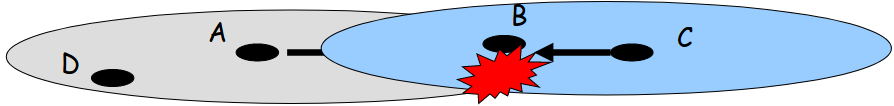
\includegraphics[scale=0.4]{SINR1}
  \caption{An example of a collision detection}
\end{figure}

In this formula $P^{X}_{transmit}$ represents the power transmission of X, and
$d^{\alpha}_{XY}$ is the \textit{SoI} between $X$ and $Y$. The noise ($N$) is
somehow a fixed value.

The nodes position and the signal interferences cause communication problems in
wireless networks, e.g. the \textbf{hidden terminal problem} and the \textbf{
  exposed terminal problem}, that will be explained in the next part.

\section{Communication problems with wireless networks}

As already mentioned, there are problems with wireless networks related to the
nodes' position and the strenght of the signal that will be explained here.

\subsection{Hidden terminal problem}

The hidden node problem occurs when a node is visible from a wireless access
point (AP) but not from other nodes communicating with that AP, due to
difficulties in the media access control sublayer.

\begin{figure}[t]
  \centering
  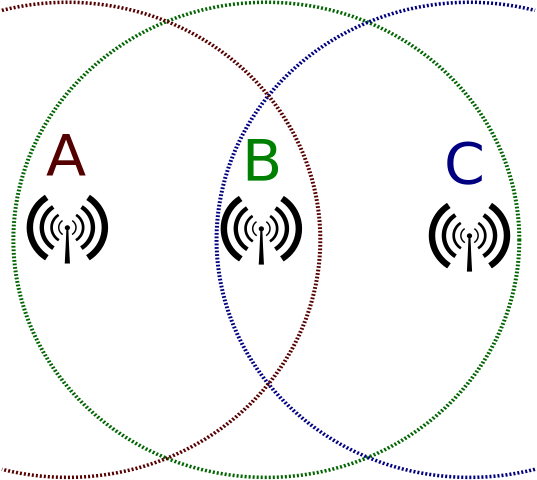
\includegraphics[scale=0.25]{WifiHiddenStationProblem}
  \caption[Hidden terminal problem]{Hidden terminal problem. Station A can
    communicate with Station B. Station C can also communicate with Station B.
    However, Stations A and C cannot communicate with each other since they
    cannot sense each other on the network, because they are out of range of
    each other.}
\end{figure}

\subsection{Exposed terminal problem}

Exposed node problem occurs when a node is prevented from sending packets to
other nodes because of a neightboring transmitter.

\begin{figure}[t]
  \centering
  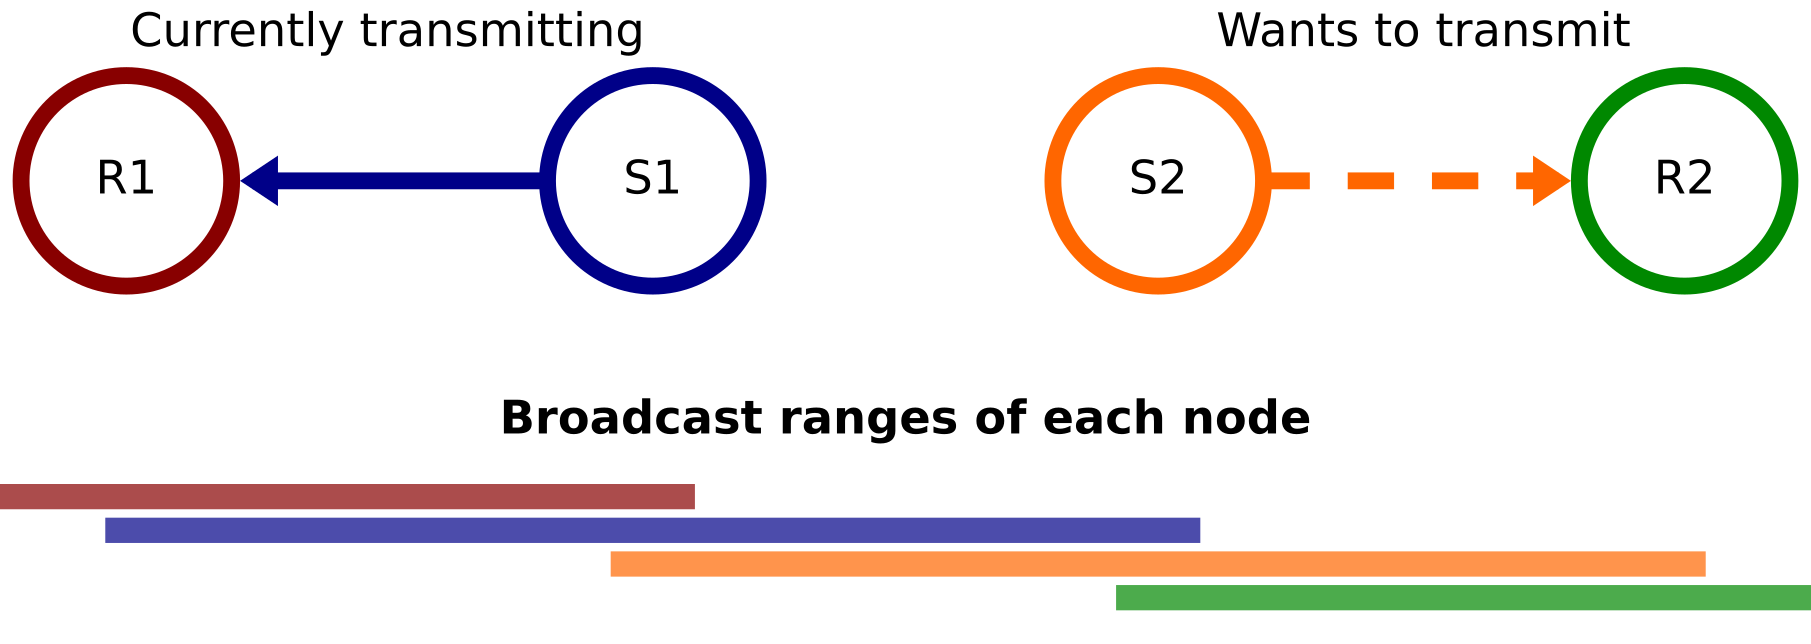
\includegraphics[scale=0.8]{WifiExposedStationProblem}
  \caption[Exposed terminal problem]{Exposed terminal problem. Station S2
    wants to communicate with R2, but has sensed S1 that's currently
    transmitting to R1 so it doesn't trasmit for not causing a collision. In
    this case, though, S2 should not defer trasmission to R2 because this won't
    create any interference with S1's trasmission.}
\end{figure}

\subsection{MACAW} \todo{This part is very confused, since the slides are a
  clusterfuck of infomation throwed randomly. Please check out \underline{very
    closely} and critically this content because I'm not sure of what I'm
  writing!}

Given that wireless MAC proved to be non-trivial, in 1994 a research lead by
Bhargavan made MACAW (\textit{Multiple Access with Collision Avoidance for
  Wireless}) that now is used for congestion avoidance. It has the same
operating principle of 802.11, and it's widely used in ad hoc networks.
MACAW helps solving the hidden terminal problem, but not the exposed terminal
problem.

\paragraph*{How it works} 
MACAW uses CTS and RTS packets to knowing if the channel is free to be used to
transmit new data.

\subparagraph*{RTS} \textit{Request to Send} is a frame sent by the
sender to the receiver before starting a trasmission that asks if there are no
curring tramission that could interfere with the new one

\subparagraph*{CTS} \textit{Clear To Send} is a frame sent by the receiver
that informs the sender that there is a possibility to use the channel to start
a new transmission.

\begin{figure}[t]
  \centering
  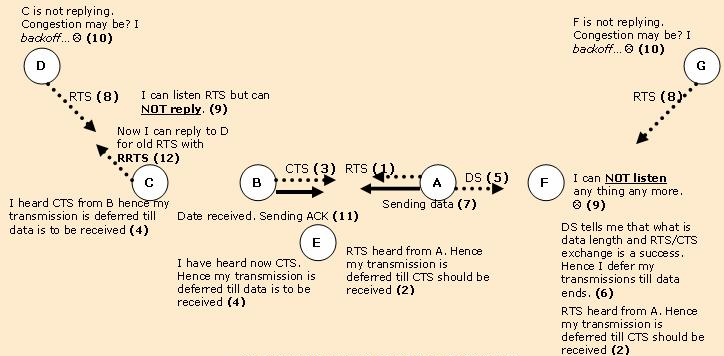
\includegraphics[scale=0.75]{MACAW}
  \caption{A schema describing an example of how MACAW works}
\end{figure}


\subparagraph*{Contention window} MACAW uses contention windows (\textit{cw}) to
determine the packet transmission rate. Whan a node fails to receive CTS in
response to its RTS it multiplies his contention window by $1.5$. This approach
is less agressive than 802.11, which multiplies by $2$. When a node successfully
completes a transfer, it reduces the contention window by $1$\footnote{That
  reduction could be a little too conservative.}. This avoids wild oscillation
of the contention window when congestion is high.
The congestion window helps with the fairness: when a node transmits the
packet it appends its current congestion windows, that is used by the others
for future transmission output.

\paragraph*{Fairness}
There are two main ways to establish fairness in MACAW, via \textit{Weighted fair queuing} and via \textit{Distributed fair scheduling (DFS)}.

\subparagraph*{Weighted fair queuing} Each node has a weight in order to have a bandwith usage proportional to it

\subparagraph*{DFS} The \textit{Distributed fair scheduling}:
\begin{itemize}
\item chooses backoff intervals proportional to packet size/weight
\item works well on LAN
\item always include some randomness
\end{itemize}

\paragraph*{Scanning} Scanning it obviously join, find and inizialize a network.
It can be of 2 typologies:
\begin{itemize}
\item active: the client actively search for beacons
\item passive: the AP sends beacons continuosly
\end{itemize}

\section{MAC for 802.11}
\paragraph*{802.11} The 802.11 protocol is used mostly indoor, it uses three
bands (900 MHz, 2.4GHz, 5GHz) and its applications are related to nomadic
internet access, portable computind and ad-hoc networking.
802.11 has two types of configurations:
\begin{itemize}
\item with a base station (control station, access point)
\item ad-hoc networking (poit-to-point)
\end{itemize}

\paragraph*{Steps for establishing a connection}
The steps for establishing a connection through the MAC protocol in 802.11 are:
\begin{enumerate}
\item[1] DIFS (\textit{Distributed Inter Frame Space}): time where the channel
  has to be free. If a node gains access to the channel goes to step 2a,
  otherwise to step 2b.
\item[2a] Data transmission
\item[2b] NAV (\textit{Network Allocation Vector}): time where the others have
  to wait before starting another transmission
\item[3] SIFS (\textit{Short Inter Frame Space}): time where the channel has to
  be free
\item[4] MAC ACK
\end{enumerate}

\subsection{Channel connection \& priorities}
Channel contentions can be of the following typologies:
\begin{itemize}
\item SIFS
\item PIFS (only with polling schema)
\item DIFS
\end{itemize}

The contention time starts before the next frame and after SIFS/PIFS/DIFS
occurs.
The packages trasmission order is the following:
\begin{AutoMultiColEnumerate}
\item DIFS
\item RTS
\item SIFS
\item CTS
\item SIFS
\item Data
\item SIFS
\item ACK
\end{AutoMultiColEnumerate}

\subsection{Access methods}
802.11 has different access methods:
\begin{itemize}
\item CSMA/CA (mandatory)
\item RTS/CTS (optional)
\item PCF (polling the AP) (optional)
\end{itemize}

\paragraph*{CSMA} CSMA doesn't entirely solve the hidden/exposed terminal
problem. The CSMA doesn't work well with the hidden terminal, so a CA
(collision avoidance) solution is used. This adds two packets before data
transmission, RTS and CTS. These packets are very little, thus fast to transmit.

\subparagraph*{Congestion avoidance} The congestion avoidance works in this way:
\begin{itemize}
\item DCF: distributed control function
\item Countdown of random back off suspended if the medium is busy (it's not
  resetted!)
\item The CW (contention window) is \underline{larger}\footnote{Large $cw$ cause
  large overhead} when there are many nodes, \underline{smaller} if fewer. When
  a node fails to receive CTS in response to its RTS, it increases the
  contention windows $x2$.
\end{itemize}

\paragraph*{PCF} With this access method the AP announces it in the beacons.
After associations frames the node announces to the AP whether it's pollable
and capable to transmit during the contention free period (CFP).

\section{Power Management}
Stations are allowed to go to sleep and this state is saved in the AP memory. Pay attentions to the fact the the energy a node consumes to wake up is more thant the one it uses to stay asleep, if it wakes up too often. Sleep is inteded for long times.

When a node sleeps, the packets for it are buffered in the AP. When it wakes up, it downloads all the packages not yet received. TSF (\textit{time synchronization function)} assures AP and power save stations are synchronized.
